% REV01 Tue 22 Jun 2021 10:54:17 WIB
% START Tue 04 May 2021 13:55:16 WIB

\chapter{TRACKING THE BIRD OF PREY}

The two lime merchants, with their escort, entered the dominions of
Miss Abbey Potterson, to whom their escort (presenting them and their
pretended business over the half-door of the bar, in a confidential
way) preferred his figurative request that ‘a mouthful of fire’ might
be lighted in Cosy. Always well disposed to assist the constituted
authorities, Miss Abbey bade Bob Gliddery attend the gentlemen to
that retreat, and promptly enliven it with fire and gaslight. Of this
commission the bare-armed Bob, leading the way with a flaming wisp of
paper, so speedily acquitted himself, that Cosy seemed to leap out of a
dark sleep and embrace them warmly, the moment they passed the lintels
of its hospitable door.

‘They burn sherry very well here,’ said Mr Inspector, as a piece of
local intelligence. ‘Perhaps you gentlemen might like a bottle?’

The answer being By all means, Bob Gliddery received his instructions
from Mr Inspector, and departed in a becoming state of alacrity
engendered by reverence for the majesty of the law.

‘It’s a certain fact,’ said Mr Inspector, ‘that this man we have
received our information from,’ indicating Riderhood with his thumb over
his shoulder, ‘has for some time past given the other man a bad name
arising out of your lime barges, and that the other man has been avoided
in consequence. I don’t say what it means or proves, but it’s a certain
fact. I had it first from one of the opposite sex of my acquaintance,’
vaguely indicating Miss Abbey with his thumb over his shoulder, ‘down
away at a distance, over yonder.’

Then probably Mr Inspector was not quite unprepared for their visit that
evening? Lightwood hinted.

‘Well you see,’ said Mr Inspector, ‘it was a question of making a move.
It’s of no use moving if you don’t know what your move is. You had
better by far keep still. In the matter of this lime, I certainly had
an idea that it might lie betwixt the two men; I always had that idea.
Still I was forced to wait for a start, and I wasn’t so lucky as to get
a start. This man that we have received our information from, has got
a start, and if he don’t meet with a check he may make the running and
come in first. There may turn out to be something considerable for him
that comes in second, and I don’t mention who may or who may not try
for that place. There’s duty to do, and I shall do it, under any
circumstances; to the best of my judgment and ability.’

‘Speaking as a shipper of lime--’ began Eugene.

‘Which no man has a better right to do than yourself, you know,’ said Mr
Inspector.

‘I hope not,’ said Eugene; ‘my father having been a shipper of lime
before me, and my grandfather before him--in fact we having been a
family immersed to the crowns of our heads in lime during several
generations--I beg to observe that if this missing lime could be got
hold of without any young female relative of any distinguished gentleman
engaged in the lime trade (which I cherish next to my life) being
present, I think it might be a more agreeable proceeding to the
assisting bystanders, that is to say, lime-burners.’

‘I also,’ said Lightwood, pushing his friend aside with a laugh, ‘should
much prefer that.’

‘It shall be done, gentlemen, if it can be done conveniently,’ said
Mr Inspector, with coolness. ‘There is no wish on my part to cause any
distress in that quarter. Indeed, I am sorry for that quarter.’

‘There was a boy in that quarter,’ remarked Eugene. ‘He is still there?’

‘No,’ said Mr Inspector. ‘He has quitted those works. He is otherwise
disposed of.’

‘Will she be left alone then?’ asked Eugene.

‘She will be left,’ said Mr Inspector, ‘alone.’

Bob’s reappearance with a steaming jug broke off the conversation. But
although the jug steamed forth a delicious perfume, its contents had not
received that last happy touch which the surpassing finish of the Six
Jolly Fellowship Porters imparted on such momentous occasions. Bob
carried in his left hand one of those iron models of sugar-loaf hats,
before mentioned, into which he emptied the jug, and the pointed end of
which he thrust deep down into the fire, so leaving it for a few moments
while he disappeared and reappeared with three bright drinking-glasses.
Placing these on the table and bending over the fire, meritoriously
sensible of the trying nature of his duty, he watched the wreaths of
steam, until at the special instant of projection he caught up the iron
vessel and gave it one delicate twirl, causing it to send forth one
gentle hiss. Then he restored the contents to the jug; held over the
steam of the jug, each of the three bright glasses in succession;
finally filled them all, and with a clear conscience awaited the
applause of his fellow-creatures.

It was bestowed (Mr Inspector having proposed as an appropriate
sentiment ‘The lime trade!’) and Bob withdrew to report the
commendations of the guests to Miss Abbey in the bar. It may be here
in confidence admitted that, the room being close shut in his absence,
there had not appeared to be the slightest reason for the elaborate
maintenance of this same lime fiction. Only it had been regarded by Mr
Inspector as so uncommonly satisfactory, and so fraught with mysterious
virtues, that neither of his clients had presumed to question it.

Two taps were now heard on the outside of the window. Mr Inspector,
hastily fortifying himself with another glass, strolled out with a
noiseless foot and an unoccupied countenance. As one might go to survey
the weather and the general aspect of the heavenly bodies.

‘This is becoming grim, Mortimer,’ said Eugene, in a low voice. ‘I don’t
like this.’

‘Nor I’ said Lightwood. ‘Shall we go?’

‘Being here, let us stay. You ought to see it out, and I won’t leave
you. Besides, that lonely girl with the dark hair runs in my head. It
was little more than a glimpse we had of her that last time, and yet
I almost see her waiting by the fire to-night. Do you feel like a dark
combination of traitor and pickpocket when you think of that girl?’

‘Rather,’ returned Lightwood. ‘Do you?’

‘Very much so.’

Their escort strolled back again, and reported. Divested of its various
lime-lights and shadows, his report went to the effect that Gaffer was
away in his boat, supposed to be on his old look-out; that he had been
expected last high-water; that having missed it for some reason or
other, he was not, according to his usual habits at night, to be counted
on before next high-water, or it might be an hour or so later; that his
daughter, surveyed through the window, would seem to be so expecting
him, for the supper was not cooking, but set out ready to be cooked;
that it would be high-water at about one, and that it was now barely
ten; that there was nothing to be done but watch and wait; that the
informer was keeping watch at the instant of that present reporting, but
that two heads were better than one (especially when the second was
Mr Inspector’s); and that the reporter meant to share the watch. And
forasmuch as crouching under the lee of a hauled-up boat on a night when
it blew cold and strong, and when the weather was varied with blasts of
hail at times, might be wearisome to amateurs, the reporter closed with
the recommendation that the two gentlemen should remain, for a while at
any rate, in their present quarters, which were weather-tight and warm.

They were not inclined to dispute this recommendation, but they wanted
to know where they could join the watchers when so disposed. Rather than
trust to a verbal description of the place, which might mislead, Eugene
(with a less weighty sense of personal trouble on him than he usually
had) would go out with Mr Inspector, note the spot, and come back.

On the shelving bank of the river, among the slimy stones of a
causeway--not the special causeway of the Six Jolly Fellowships, which
had a landing-place of its own, but another, a little removed, and
very near to the old windmill which was the denounced man’s
dwelling-place--were a few boats; some, moored and already beginning to
float; others, hauled up above the reach of the tide. Under one of these
latter, Eugene’s companion disappeared. And when Eugene had observed its
position with reference to the other boats, and had made sure that he
could not miss it, he turned his eyes upon the building where, as he had
been told, the lonely girl with the dark hair sat by the fire.

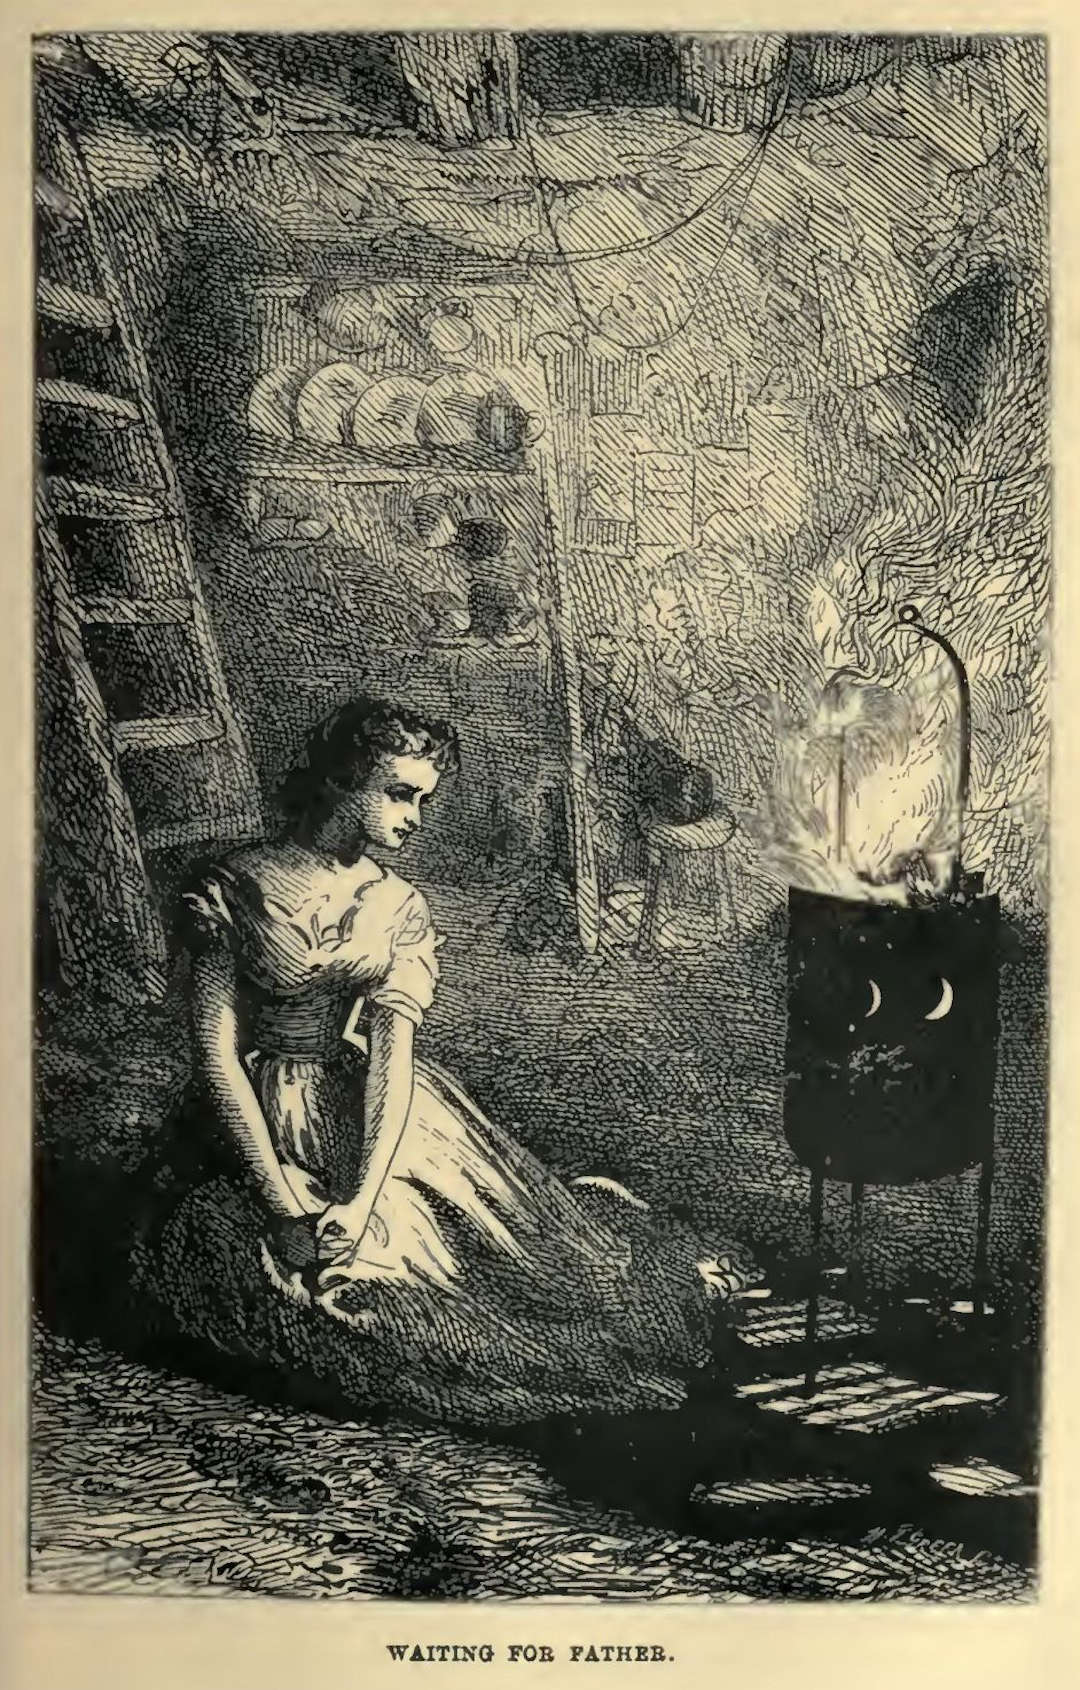
\includegraphics[scale=1.9]{01-13-01}

He could see the light of the fire shining through the window. Perhaps
it drew him on to look in. Perhaps he had come out with the express
intention. That part of the bank having rank grass growing on it, there
was no difficulty in getting close, without any noise of footsteps: it
was but to scramble up a ragged face of pretty hard mud some three or
four feet high and come upon the grass and to the window. He came to the
window by that means.

She had no other light than the light of the fire. The unkindled lamp
stood on the table. She sat on the ground, looking at the brazier, with
her face leaning on her hand. There was a kind of film or flicker on
her face, which at first he took to be the fitful firelight; but, on a
second look, he saw that she was weeping. A sad and solitary spectacle,
as shown him by the rising and the falling of the fire.

It was a little window of but four pieces of glass, and was not
curtained; he chose it because the larger window near it was. It showed
him the room, and the bills upon the wall respecting the drowned people
starting out and receding by turns. But he glanced slightly at them,
though he looked long and steadily at her. A deep rich piece of colour,
with the brown flush of her cheek and the shining lustre of her hair,
though sad and solitary, weeping by the rising and the falling of the
fire.

She started up. He had been so very still that he felt sure it was not
he who had disturbed her, so merely withdrew from the window and stood
near it in the shadow of the wall. She opened the door, and said in an
alarmed tone, ‘Father, was that you calling me?’ And again, ‘Father!’
And once again, after listening, ‘Father! I thought I heard you call me
twice before!’

No response. As she re-entered at the door, he dropped over the bank and
made his way back, among the ooze and near the hiding-place, to Mortimer
Lightwood: to whom he told what he had seen of the girl, and how this
was becoming very grim indeed.

‘If the real man feels as guilty as I do,’ said Eugene, ‘he is
remarkably uncomfortable.’

‘Influence of secrecy,’ suggested Lightwood.

‘I am not at all obliged to it for making me Guy Fawkes in the vault and
a Sneak in the area both at once,’ said Eugene. ‘Give me some more of
that stuff.’

Lightwood helped him to some more of that stuff, but it had been
cooling, and didn’t answer now.

‘Pooh,’ said Eugene, spitting it out among the ashes. ‘Tastes like the
wash of the river.’

‘Are you so familiar with the flavour of the wash of the river?’

‘I seem to be to-night. I feel as if I had been half drowned, and
swallowing a gallon of it.’

‘Influence of locality,’ suggested Lightwood.

‘You are mighty learned to-night, you and your influences,’ returned
Eugene. ‘How long shall we stay here?’

‘How long do you think?’

‘If I could choose, I should say a minute,’ replied Eugene, ‘for the
Jolly Fellowship Porters are not the jolliest dogs I have known. But
I suppose we are best here until they turn us out with the other
suspicious characters, at midnight.’

Thereupon he stirred the fire, and sat down on one side of it. It struck
eleven, and he made believe to compose himself patiently. But gradually
he took the fidgets in one leg, and then in the other leg, and then in
one arm, and then in the other arm, and then in his chin, and then in
his back, and then in his forehead, and then in his hair, and then in
his nose; and then he stretched himself recumbent on two chairs, and
groaned; and then he started up.

‘Invisible insects of diabolical activity swarm in this place. I am
tickled and twitched all over. Mentally, I have now committed a burglary
under the meanest circumstances, and the myrmidons of justice are at my
heels.’

‘I am quite as bad,’ said Lightwood, sitting up facing him, with a
tumbled head; after going through some wonderful evolutions, in which
his head had been the lowest part of him. ‘This restlessness began with
me, long ago. All the time you were out, I felt like Gulliver with the
Lilliputians firing upon him.’

‘It won’t do, Mortimer. We must get into the air; we must join our dear
friend and brother, Riderhood. And let us tranquillize ourselves by
making a compact. Next time (with a view to our peace of mind) we’ll
commit the crime, instead of taking the criminal. You swear it?’

‘Certainly.’

‘Sworn! Let Tippins look to it. Her life’s in danger.’

Mortimer rang the bell to pay the score, and Bob appeared to transact
that business with him: whom Eugene, in his careless extravagance, asked
if he would like a situation in the lime-trade?

‘Thankee sir, no sir,’ said Bob. ‘I’ve a good sitiwation here, sir.’

‘If you change your mind at any time,’ returned Eugene, ‘come to me at
my works, and you’ll always find an opening in the lime-kiln.’

‘Thankee sir,’ said Bob.

‘This is my partner,’ said Eugene, ‘who keeps the books and attends to
the wages. A fair day’s wages for a fair day’s work is ever my partner’s
motto.’

‘And a very good ‘un it is, gentlemen,’ said Bob, receiving his fee, and
drawing a bow out of his head with his right hand, very much as he would
have drawn a pint of beer out of the beer engine.

‘Eugene,’ Mortimer apostrophized him, laughing quite heartily when they
were alone again, ‘how CAN you be so ridiculous?’

‘I am in a ridiculous humour,’ quoth Eugene; ‘I am a ridiculous fellow.
Everything is ridiculous. Come along!’

It passed into Mortimer Lightwood’s mind that a change of some sort,
best expressed perhaps as an intensification of all that was wildest and
most negligent and reckless in his friend, had come upon him in the last
half-hour or so. Thoroughly used to him as he was, he found something
new and strained in him that was for the moment perplexing. This passed
into his mind, and passed out again; but he remembered it afterwards.

‘There’s where she sits, you see,’ said Eugene, when they were standing
under the bank, roared and riven at by the wind. ‘There’s the light of
her fire.’

‘I’ll take a peep through the window,’ said Mortimer.

‘No, don’t!’ Eugene caught him by the arm. ‘Best, not make a show of
her. Come to our honest friend.’

He led him to the post of watch, and they both dropped down and crept
under the lee of the boat; a better shelter than it had seemed before,
being directly contrasted with the blowing wind and the bare night.

‘Mr Inspector at home?’ whispered Eugene.

‘Here I am, sir.’

‘And our friend of the perspiring brow is at the far corner there? Good.
Anything happened?’

‘His daughter has been out, thinking she heard him calling, unless it
was a sign to him to keep out of the way. It might have been.’

‘It might have been Rule Britannia,’ muttered Eugene, ‘but it wasn’t.
Mortimer!’

‘Here!’ (On the other side of Mr Inspector.)

‘Two burglaries now, and a forgery!’

With this indication of his depressed state of mind, Eugene fell silent.

They were all silent for a long while. As it got to be flood-tide, and
the water came nearer to them, noises on the river became more frequent,
and they listened more. To the turning of steam-paddles, to the clinking
of iron chain, to the creaking of blocks, to the measured working
of oars, to the occasional violent barking of some passing dog on
shipboard, who seemed to scent them lying in their hiding-place. The
night was not so dark but that, besides the lights at bows and mastheads
gliding to and fro, they could discern some shadowy bulk attached; and
now and then a ghostly lighter with a large dark sail, like a warning
arm, would start up very near them, pass on, and vanish. At this time
of their watch, the water close to them would be often agitated by some
impulsion given it from a distance. Often they believed this beat and
plash to be the boat they lay in wait for, running in ashore; and again
and again they would have started up, but for the immobility with which
the informer, well used to the river, kept quiet in his place.

The wind carried away the striking of the great multitude of city
church clocks, for those lay to leeward of them; but there were bells to
windward that told them of its being One--Two--Three. Without that aid
they would have known how the night wore, by the falling of the tide,
recorded in the appearance of an ever-widening black wet strip of shore,
and the emergence of the paved causeway from the river, foot by foot.

As the time so passed, this slinking business became a more and more
precarious one. It would seem as if the man had had some intimation of
what was in hand against him, or had taken fright? His movements might
have been planned to gain for him, in getting beyond their reach, twelve
hours’ advantage? The honest man who had expended the sweat of his brow
became uneasy, and began to complain with bitterness of the proneness of
mankind to cheat him--him invested with the dignity of Labour!

Their retreat was so chosen that while they could watch the river, they
could watch the house. No one had passed in or out, since the daughter
thought she heard the father calling. No one could pass in or out
without being seen.

‘But it will be light at five,’ said Mr Inspector, ‘and then WE shall be
seen.’

‘Look here,’ said Riderhood, ‘what do you say to this? He may have
been lurking in and out, and just holding his own betwixt two or three
bridges, for hours back.’

‘What do you make of that?’ said Mr Inspector. Stoical, but
contradictory.

‘He may be doing so at this present time.’

‘What do you make of that?’ said Mr Inspector.

‘My boat’s among them boats here at the cause’ay.’

‘And what do you make of your boat?’ said Mr Inspector.

‘What if I put off in her and take a look round? I know his ways, and
the likely nooks he favours. I know where he’d be at such a time of the
tide, and where he’d be at such another time. Ain’t I been his pardner?
None of you need show. None of you need stir. I can shove her off
without help; and as to me being seen, I’m about at all times.’

‘You might have given a worse opinion,’ said Mr Inspector, after brief
consideration. ‘Try it.’

‘Stop a bit. Let’s work it out. If I want you, I’ll drop round under the
Fellowships and tip you a whistle.’

‘If I might so far presume as to offer a suggestion to my honourable and
gallant friend, whose knowledge of naval matters far be it from me to
impeach,’ Eugene struck in with great deliberation, ‘it would be, that
to tip a whistle is to advertise mystery and invite speculation.
My honourable and gallant friend will, I trust, excuse me, as an
independent member, for throwing out a remark which I feel to be due to
this house and the country.’

‘Was that the T’other Governor, or Lawyer Lightwood?’ asked Riderhood.
For, they spoke as they crouched or lay, without seeing one another’s
faces.

‘In reply to the question put by my honourable and gallant friend,’
said Eugene, who was lying on his back with his hat on his face, as an
attitude highly expressive of watchfulness, ‘I can have no hesitation in
replying (it not being inconsistent with the public service) that those
accents were the accents of the T’other Governor.’

‘You’ve tolerable good eyes, ain’t you, Governor? You’ve all tolerable
good eyes, ain’t you?’ demanded the informer.

All.

‘Then if I row up under the Fellowship and lay there, no need to
whistle. You’ll make out that there’s a speck of something or another
there, and you’ll know it’s me, and you’ll come down that cause’ay to
me. Understood all?’

Understood all.

‘Off she goes then!’

In a moment, with the wind cutting keenly at him sideways, he was
staggering down to his boat; in a few moments he was clear, and creeping
up the river under their own shore.

Eugene had raised himself on his elbow to look into the darkness after
him. ‘I wish the boat of my honourable and gallant friend,’ he murmured,
lying down again and speaking into his hat, ‘may be endowed
with philanthropy enough to turn bottom-upward and extinguish
him!--Mortimer.’

‘My honourable friend.’

‘Three burglaries, two forgeries, and a midnight assassination.’ Yet
in spite of having those weights on his conscience, Eugene was somewhat
enlivened by the late slight change in the circumstances of affairs. So
were his two companions. Its being a change was everything. The suspense
seemed to have taken a new lease, and to have begun afresh from a recent
date. There was something additional to look for. They were all three
more sharply on the alert, and less deadened by the miserable influences
of the place and time.

More than an hour had passed, and they were even dozing, when one of the
three--each said it was he, and he had NOT dozed--made out Riderhood
in his boat at the spot agreed on. They sprang up, came out from their
shelter, and went down to him. When he saw them coming, he dropped
alongside the causeway; so that they, standing on the causeway, could
speak with him in whispers, under the shadowy mass of the Six Jolly
Fellowship Porters fast asleep.

‘Blest if I can make it out!’ said he, staring at them.

‘Make what out? Have you seen him?’

‘No.’

‘What HAVE you seen?’ asked Lightwood. For, he was staring at them in
the strangest way.

‘I’ve seen his boat.’

‘Not empty?’

‘Yes, empty. And what’s more,--adrift. And what’s more,--with one scull
gone. And what’s more,--with t’other scull jammed in the thowels and
broke short off. And what’s more,--the boat’s drove tight by the tide
‘atwixt two tiers of barges. And what’s more,--he’s in luck again, by
George if he ain’t!’



